\documentclass[fr]{../../../../../../eplexam}

\usepackage{../../../math-FSAB1103-exam}
\usepackage[SIunits]{../../../../../../eplunits}

\hypertitle{Math\'ematique}{3}{FSAB}{1103}{2016}{Ao\^ut}{All}
{William André}
{Jean-François Remacle et Grégoire Winckelmans}

\section{Question 1 : caractéristiques}
Soit l'EDP suivante :
\[ P\fpart{u}{x} + Q\fpart{u}{y} = R\]
et la courbe $\Gamma(s)$ définie par $x(s)=r_0\cos(s)$ et $y(s)=r_0\sin(s)$ \\
On sait que l'équation des caractéristiques est de la forme $r = L\theta + B(r_0,s)$ avec $x = r\cos(\theta)$ et $y=r\sin(\theta)$. On a aussi que $u(x(s),y(s)) = u_{0} \sin^{3}(s)$.
\begin{enumerate}
	\item Déterminez $B(r_0,s)$. Dessinez le réseau des caractéritiques pour $0\leq r \leq 2r_0$ et $s=-\frac{\pi}{4};0;\frac{\pi}{4};\frac{\pi}{2}$
	\item Différentiez l'équation des caractéristiques pour obtenir la forme de $P(x,y)$ et $Q(x,y)$ \\ Rappel : $\frac{\mathrm d}{\mathrm dv} \arctan(v)=\frac{1}{(1+v^2)}$.
	\item En supposant $R=0$, déterminer la valeur de $u(\sqrt{2}r_0,\sqrt{2}r_0)$. En quelle(s) valeur(s) la solution n'est elle pas définie ?
\end{enumerate}


\begin{solution}
	\begin{enumerate}
		\item  	$$r = L\Theta +B(r_{0},s)$$
		$$B(r_{0},s) = r - L\theta$$
		$r = r_{0}$ lorsque $\theta = s$
		$$B(r_{0},s) = r_{0} - Ls$$
		$$ r = r_{0} + L(\theta - s)$$
		Le graphe des caractéristiques est disponible à la figure \ref{fig:cara}
		\begin{solfig}{cara}{Caractéristiques du problème pour différents s}
			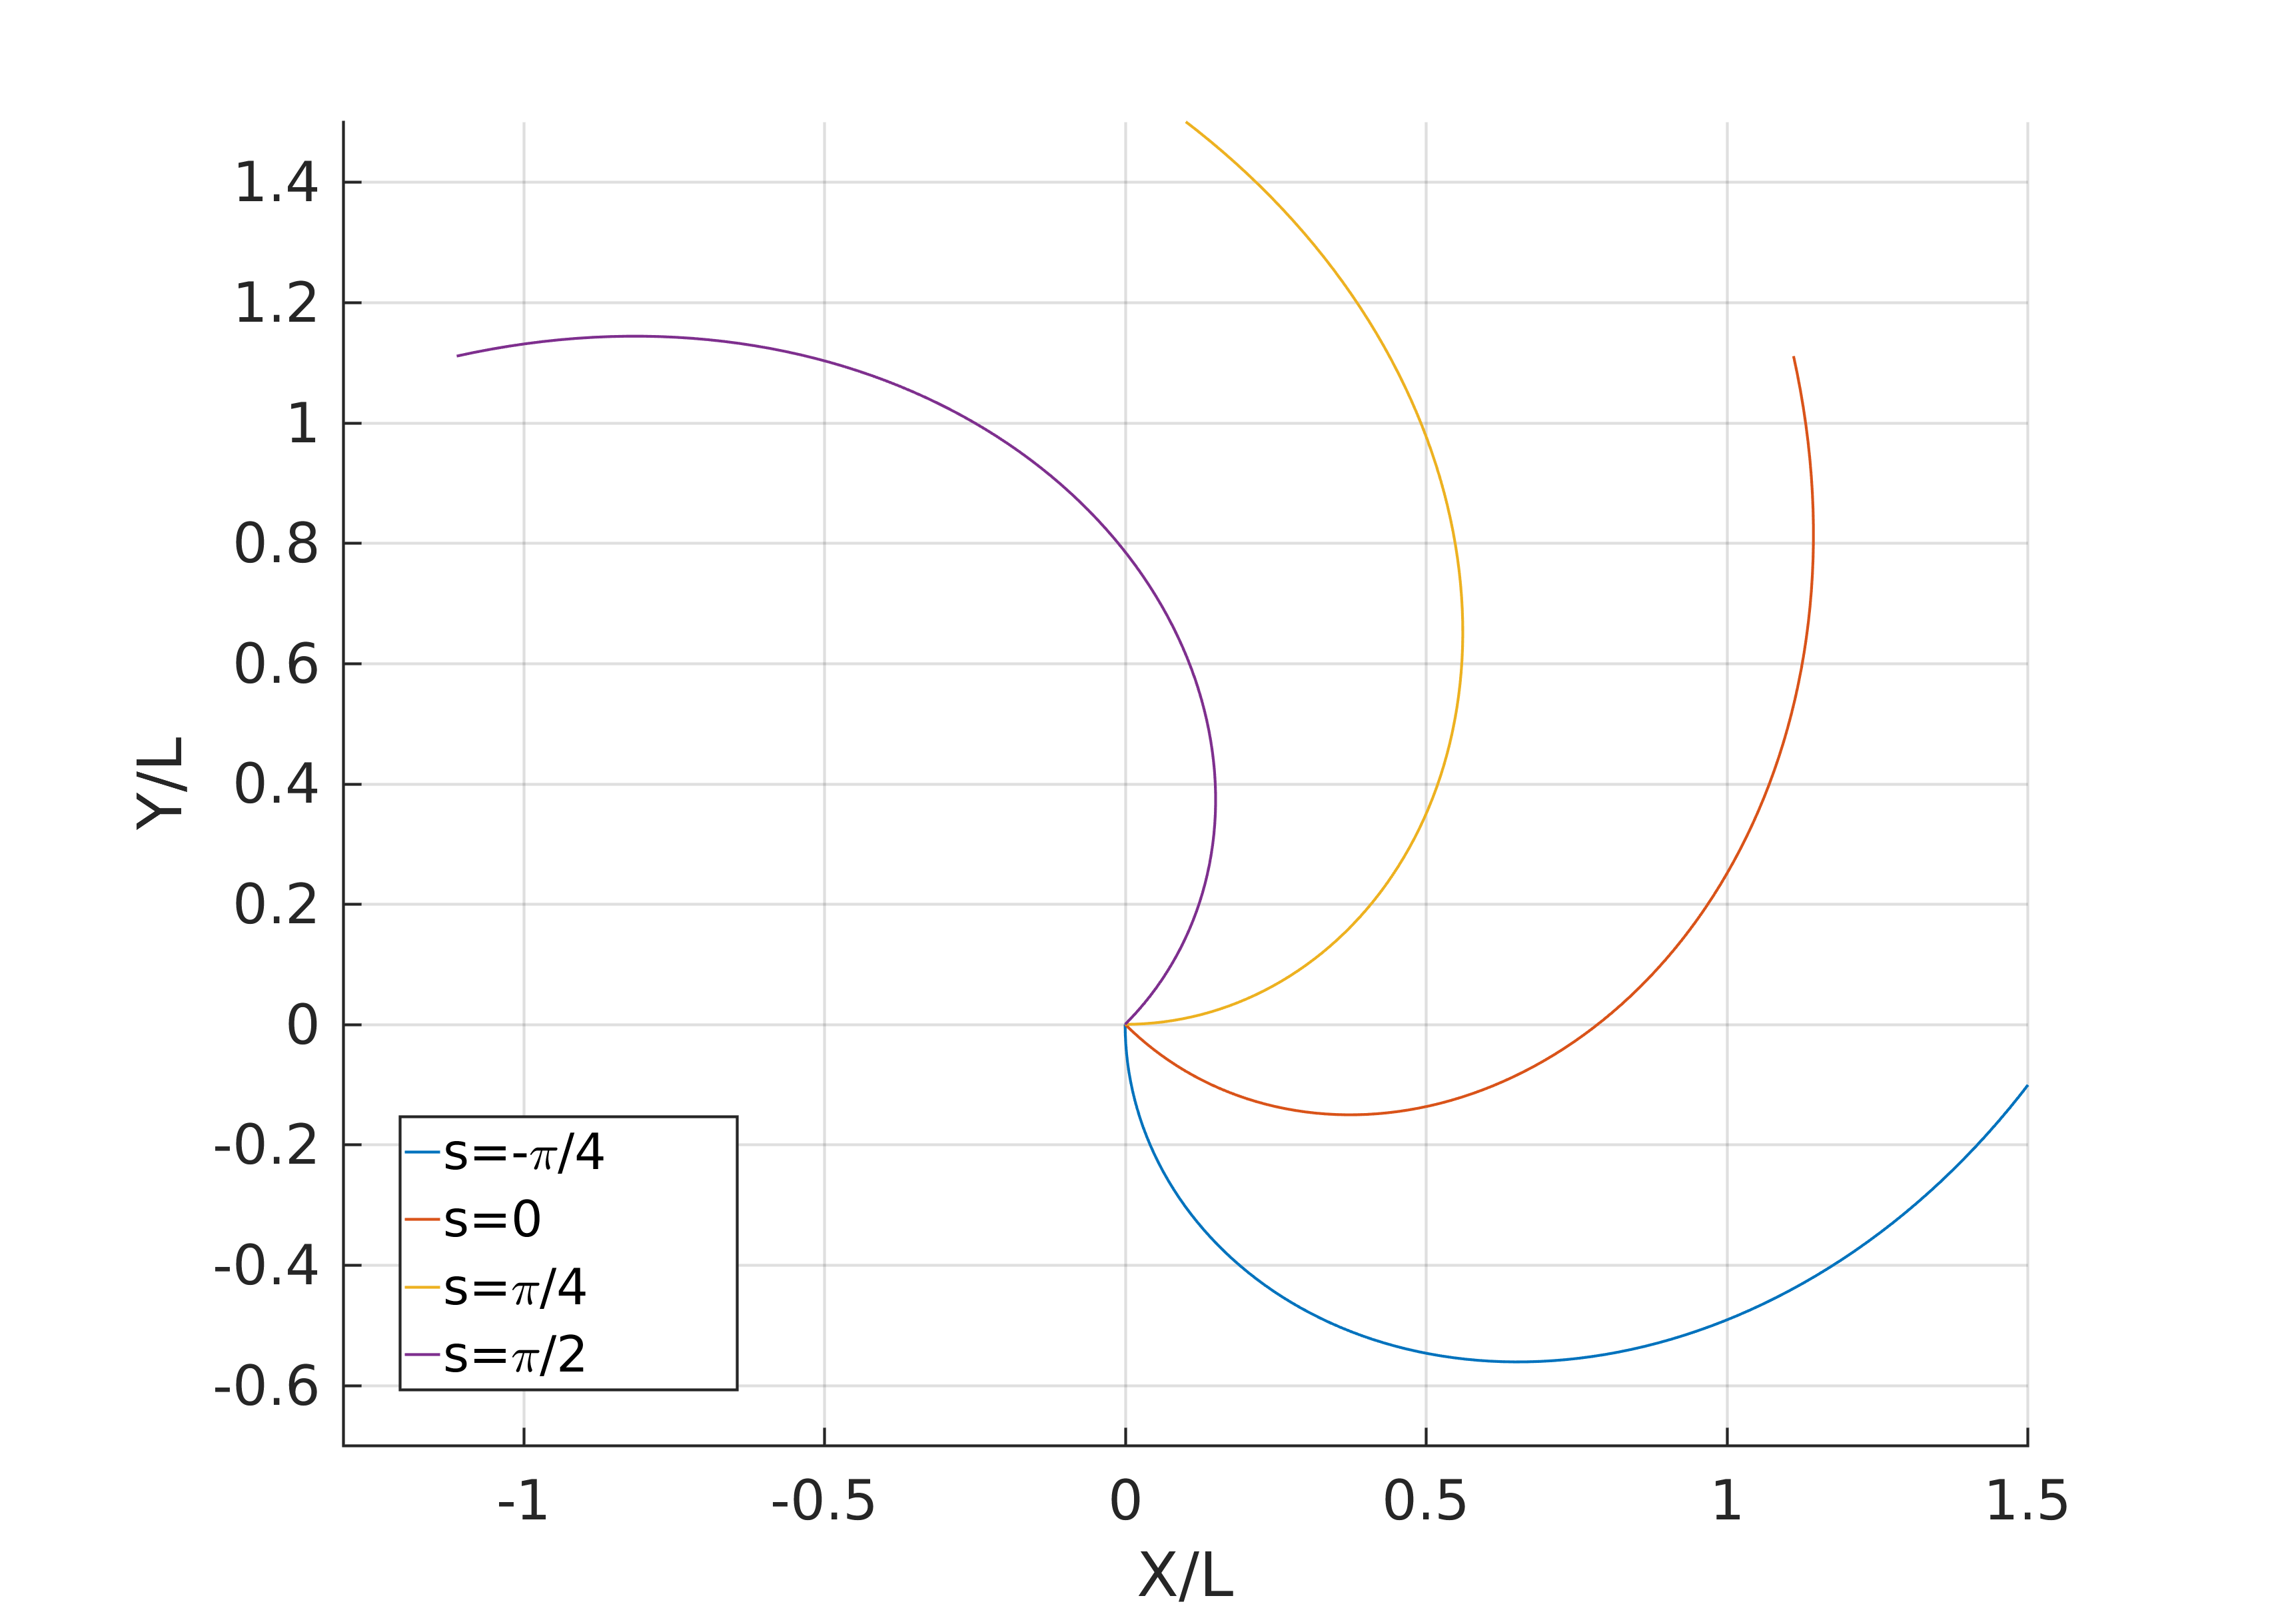
\includegraphics[width=0.8\textwidth]{spir.png}
		\end{solfig}
		
		\item 
		$$ r = r_{0} + L(\theta - s)$$
		$$\sqrt{x^{2} + y^{2}} = r_{0} + L(\arctan\left(\frac{y}{x}\right) - s)$$
		$$\cfrac{2xdx + 2ydy}{2\sqrt{x^{2} + y^{2}}} = L \cfrac{\dfrac{1}{x} dy + \dfrac{- y}{x^{2}}dx}{1+(\dfrac{y}{x})^{2}} $$
		$$\cfrac{xdx + ydy}{\sqrt{x^{2} + y^{2}}} = L \cfrac{x dy -ydx}{x^{2}+y^{2}} $$
		$$\cfrac{Lx}{\sqrt{x^{2} + y^{2}}} + y dx = \cfrac{Ly}{\sqrt{x^{2} + y^{2}}} -x dy $$
		\begin{align*}
			&P = \cfrac{Ly}{\sqrt{x^{2} + y^{2}}} -x &Q=\cfrac{Lx}{\sqrt{x^{2} + y^{2}}} + y
		\end{align*}
		
		\item Avec $R = 0$
		\begin{align*}
			u(x,y) &= u(x(s),y(s))\\
			&=u_{0} \sin^{3}(s)\\
			&=u_{0} \sin^{3}\left(\cfrac{r_{0}-r}{L} + \theta\right)\\
			&= u_{0} \sin^{3}\left(\cfrac{(1-\sqrt{4})r_{0}}{L} + \frac{\pi}{4}\right)\\
			&= u_{0} \sin^{3}\left(\frac{\pi}{4} - \frac{r_{0}}{L}\right)
		\end{align*}
		
		
	\end{enumerate}
\end{solution}

\section{Question 2 : séparation de variables}
Soit l'EDP
\[ \fpart{u}{t} = \alpha\ffpart{u}{x} + Q_0\]
avec $\alpha > 0$ constant. Le domaine est borné : $0 \leq x \leq L$. La condition initiale est $u(x,0) = u_0(\frac{2x}{L}-1)$ avec $u_0 > 0$ constant. Pour $t>0$, les conditions aux limites sont $\dfrac{\partial u }{\partial x}(0,t)=\frac{2u_0}{L}$ et $u(L,t)=u_0$
\begin{enumerate}
	\item
	De quel type d'EDP s'agit il, physiquement et mathématiquement ? Qu'est ce qu'un temps ``court'' pour le problème présent, $0 < t \ll ...$ ?

	\item
	Obtenez ensuite, mathématiquement, la solution $u(x,t)$ du problème. $u(x,t) = R(x) + \Theta (x,t)$.
	\begin{itemize}
		\item Obtenez d'abord la solution en régime. ( $R(x)$ )
		\item Obtenez ensuite la solution transitoire ( $\Theta (x,t)$ ) grace a la méthode de séparation des variables.
		\item Soit $Q_0 = \dfrac{2\alpha \cdot u_0}{L^2}$, Esquissez le graphe attendu de $\frac{u}{u_0}$ en fonction de $\frac{x}{L}$ en des temps différents : $t=0$ (CI), temps court, temps moyen, temps long, temps très long (solution de régime).
	\end{itemize}
\end{enumerate}

\begin{solution}
		\begin{enumerate}
			\item Il s'agit d'une EDP d'ordre 2, homogène et parabolique. Il s'agit d'une équation de diffusion.
			
			Un temps courts est un temps:
			$$0 < t \ll \frac{L^{2}}{\alpha} $$
			\item
			Pour la solution en régime nous avons que
			$$\fpart{u}{t} = 0$$
			donc
			$$\ffpart{u}{x} =R''(x) = - \frac{Q_{0}}{\alpha}$$
			$$R(x) = -\frac{Q_{0}}{2\alpha} x^{2} + ax + b$$
			$$R'(0) = -\frac{Q_{0}}{\alpha} *0 + a = \frac{2*u_{0}}{L}$$
			$$R(L) = -\frac{Q_{0}}{2\alpha} L^{2} + 2 u_{0} + b =u_{0}$$
			$$R(x) = -\frac{Q_{0}}{2\alpha} x^{2} + \frac{2*u_{0}}{L}x + \frac{Q_{0}}{2\alpha} L^{2} - u_{0}$$ 
			
			Pour la solution transitoire nous retombons sur une équation de diffusion comme avant sachant que le $Q_{0}$ est traité dans la solution en régime.
			
			Posons 
			$$u(x,t) = X(x)T(t)$$
			$$\frac{T'}{T} = \alpha \frac{X''}{X} = -k^{2}$$
			$$T = C \exp(-\alpha k^{2}t)$$
			$$X = A\cos(kx) + B\sin(kx)$$
			en utilisant nos condition limites:
			$$ X = A\cos(kx)$$
			avec $k=\frac{(2n-1)}{L}\frac{\pi}{2}$
			
			En utilisant notre condition initial
			
			$$R(x) +\sum_{n = 1}^{\infty} A_{n} \cos(kx) = u(x,0) = u_0(\frac{2x}{L}-1)$$
			$$\sum_{n = 1}^{\infty} A_{n} \cos(kx) = u(x,0) = u_0(\frac{2x}{L}-1) +\frac{Q_{0}}{2\alpha} x^{2} - \frac{2*u_{0}}{L}x - \frac{Q_{0}}{2\alpha} L^{2} + u_{0}$$
			
			$$\sum_{n = 1}^{\infty} A_{n} \cos(kx) = u(x,0) = 
			\frac{Q_{0}}{2\alpha} (x^{2} - L^{2})$$
			par orthogonalité
			$$A_{n}\int_{0}^{L} \cos(kx)^{2} dx= \int_{0}^{L} \frac{Q_{0}}{2\alpha} (x^{2} - L^{2}) \cos(kx)dx$$
			$$A_{n} = \int_{0}^{L} \frac{Q_{0}}{L\alpha} (x^{2}\cos(kx) - L^{2}\cos(kx))dx$$
			Intégrons chaque partie séparément
			\begin{align*}
				I_{1} &= \int_{0}^{L} x^{2}\cos(kx)dx\\
				&=\left[\frac{2x}{k^{2}} \cos(kx) +\left(\frac{x^{2}}{k}-\frac{2}{k^{3}}\right)\sin(kx)\right]_{0}^{L}\\
				&=\left( \frac{L^{2}}{k} - \frac{2}{k^{3}}\right)*-(-1)^{n}
			\end{align*}
			
			\begin{align*}
				I_{2} &=\int_{0}^{L} -L^{2} cos(kx) dx\\
				 &=\left[-\frac{L^{2}}{k} \sin(kx)\right]_{0}^{L}\\ 
				 &=\frac{L^{2}}{L} (-1)^{n}
			\end{align*}
			
			$$A_{n} = \frac{Q_{0}}{L\alpha} (I_{1} + I_{2}) = \frac{Q_{0}}{L\alpha} \frac{2}{k^{3}} (-1)^{n}$$
			$$u(x,t) = -\frac{Q_{0}}{2\alpha} x^{2} + \frac{2*u_{0}}{L}x + \frac{Q_{0}}{2\alpha} L^{2} - u_{0} +\sum_{n = 1}^{\infty} \frac{Q_{0}}{L\alpha} \frac{2}{k^{3}} (-1)^{n} \cos(kx) \exp(-\alpha k^{2}) $$
			
			Lorsque $Q_0 = \dfrac{2\alpha \cdot u_0}{L^2}$ nous obtenons
			
			$$u(x,t) = -\frac{u_{0}}{L^{2}}x^{2} + \frac{2*u_{0}}{L}x +\sum_{n = 1}^{\infty} \frac{2 u_{0}}{L^{3}} \frac{2}{k^{3}} (-1)^{n} \cos(kx) \exp(-\alpha k^{2}t) $$
			
			On trouve le graphe de la solution à la figure \ref{fig:diff}
					\begin{solfig}{diff}{u(x,t) pour différents temps.}
						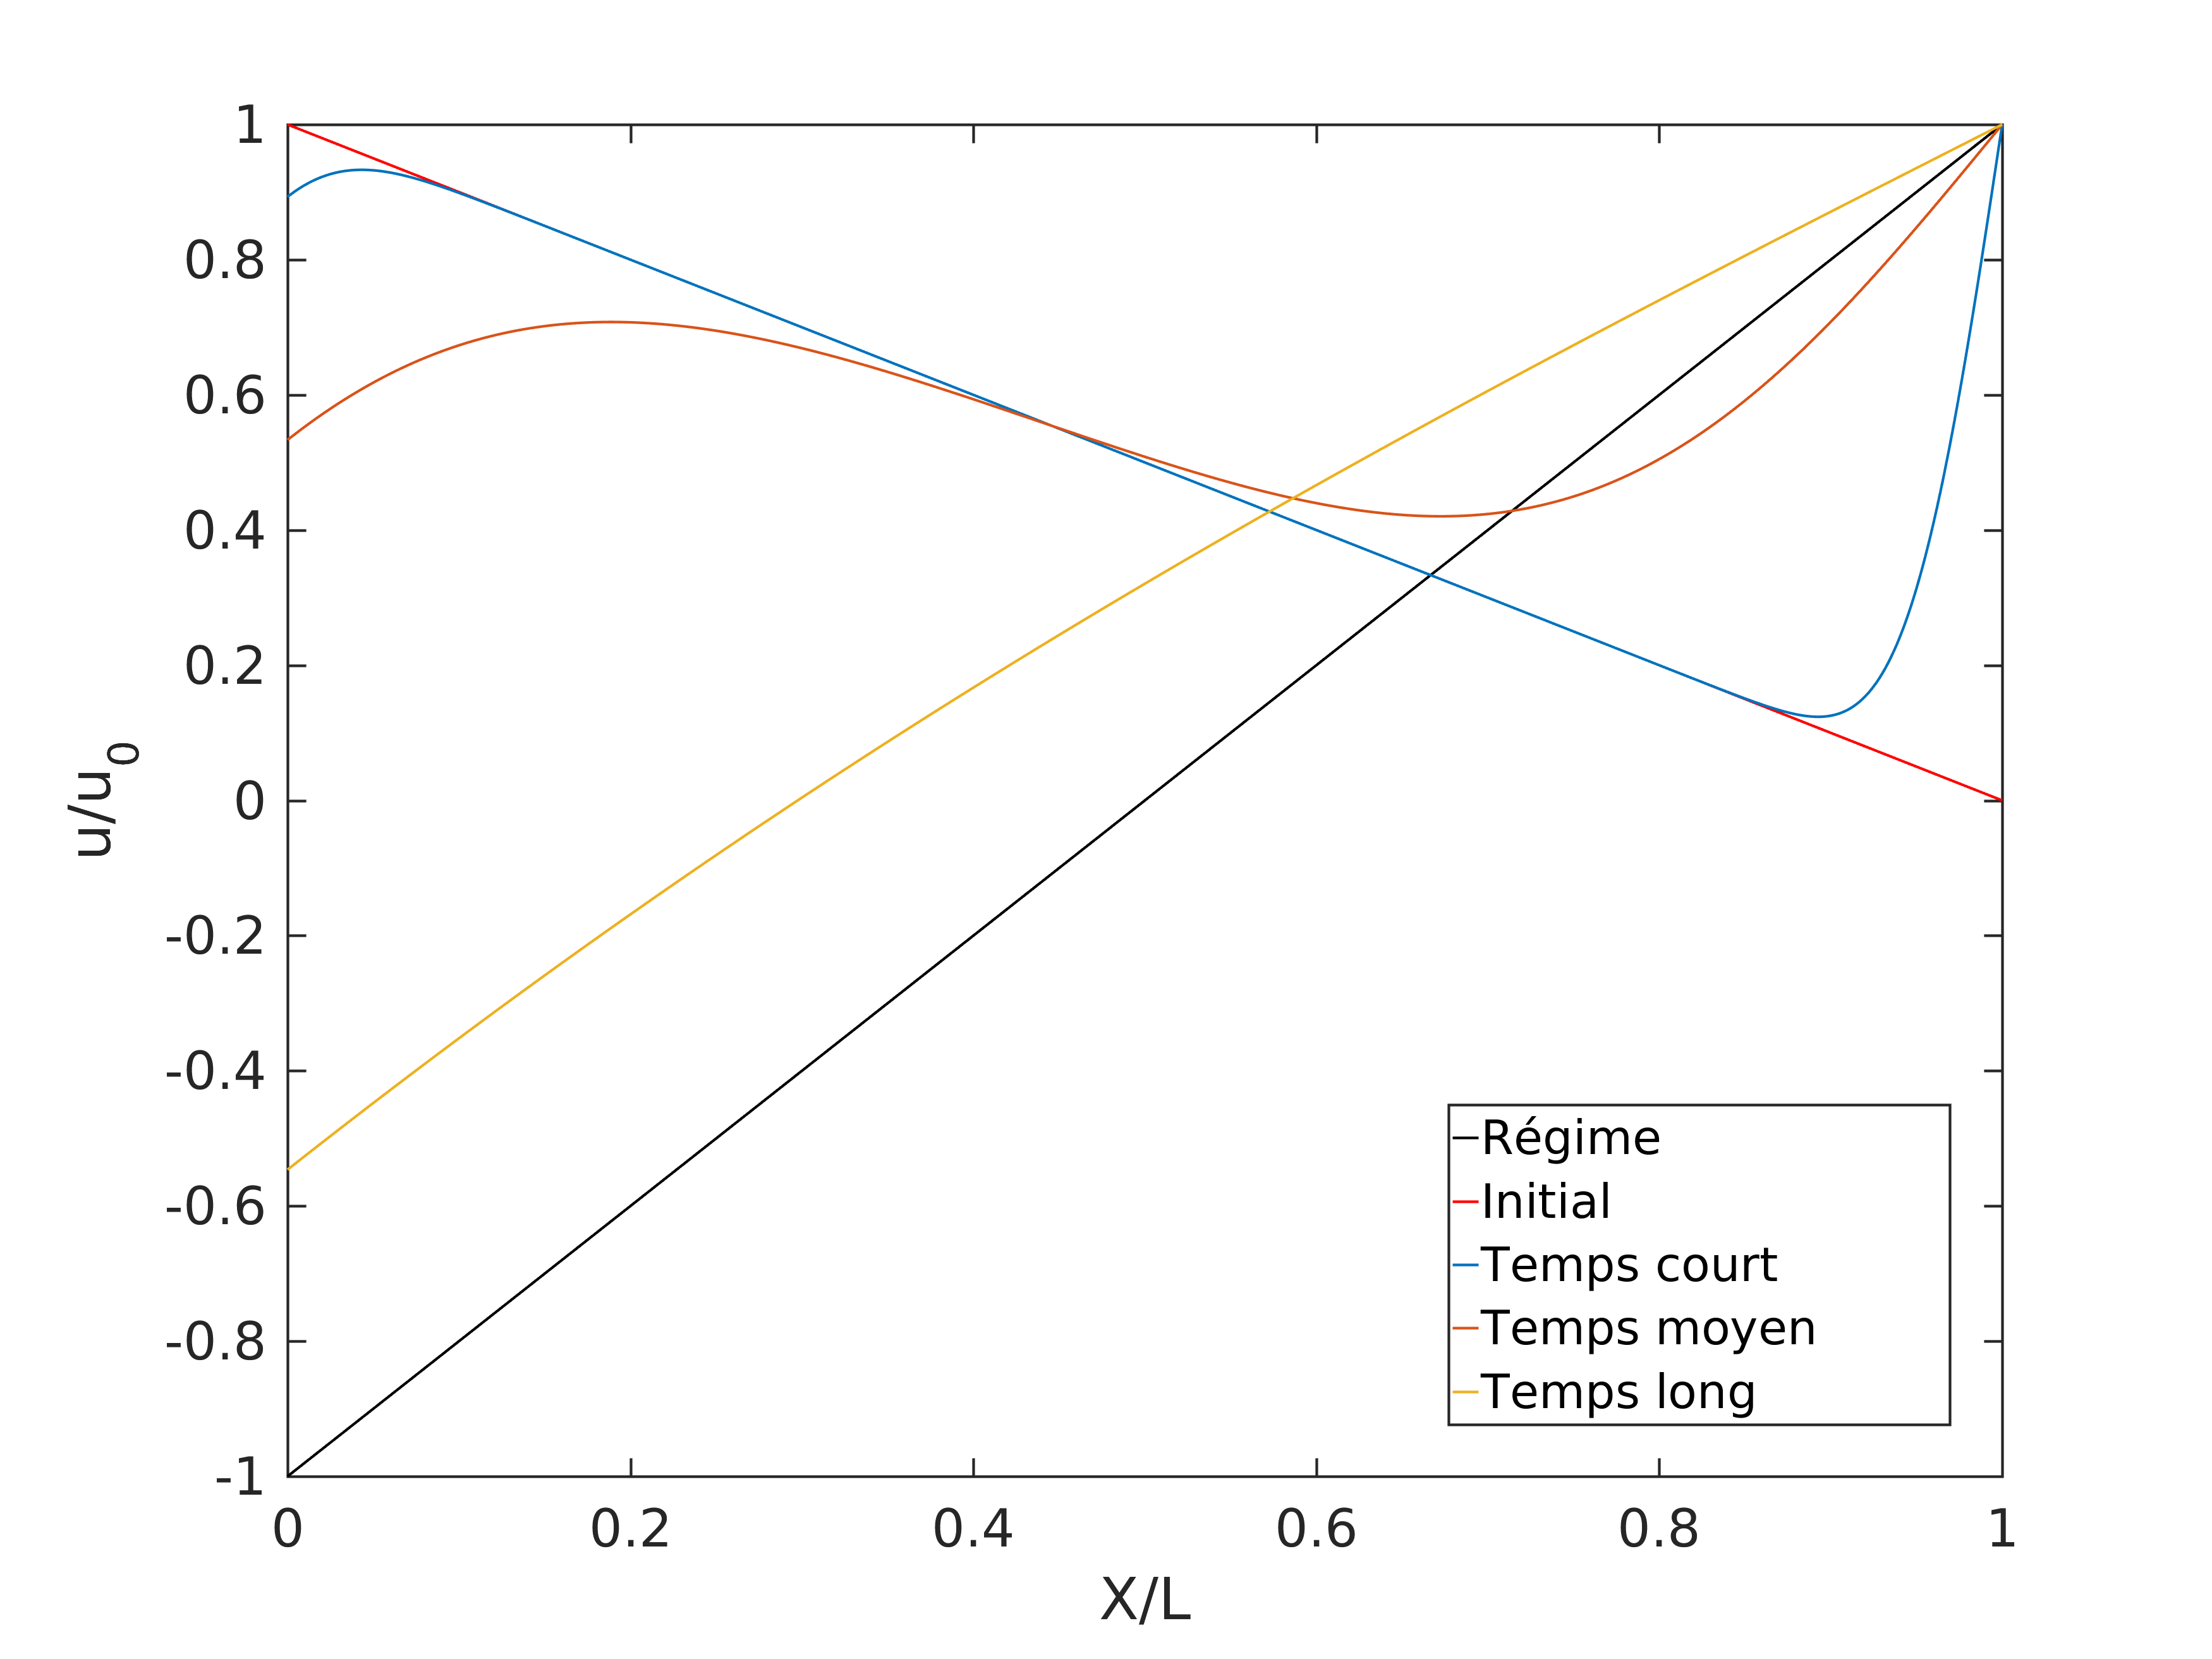
\includegraphics[width=0.8\textwidth]{diff.png}
					\end{solfig}
		\end{enumerate}
		
\end{solution}


\section{Question 3 : théorie complexe}
On définit la fonction
\[ w = \frac{1}{i} \log{\left(\frac{\sqrt{z^2-1}+i}{z}\right)}\]
\begin{enumerate}
  \item Obtenez une expression pour $\sin(w)$ en fonction de $z$ (indice : l'expression est simple)
  \item Trouver les points de branchement ( indice: $\eta =\sqrt{z^2-1}+i$ est toujours positif). Effectuer les coupure de manière à ce que la fonction soit bien définie pour z= x avec x réel et |x|>1. Définir la branche principale , nous n'utiliserons plus que celle ci pour la suite.
  \item Obtenez l'expression de $w$ pour $z=x$ pour $x>1$. Obtenez d'abord l'expression de $\eta$.
  \item Obtenez l'expression complexe de $w$ pour $z=iy$ pour $y>0$. Obtenez d'abord l'expression de $\eta$.
  \item On peut montrer (ne le faites pas ici !) que $w = \int_0^Z{\frac{1}{1+\zeta^2}d\zeta}$ avec $Z=\frac{1}{z}$ \\Obtenez le développement en série de $w$ autour de $z_0 = 0$. Quel est le rayon de convergence de la série ?
    (\textbf{Aide}: $\frac{1}{\sqrt{1+z}} = 1 - \frac{1}{2}z^1 + \frac{1.3}{2.4}z^2 - \frac{1.3.5}{2.4.6}z^3 + ...$)
\end{enumerate}

\begin{solution}
\begin{enumerate}
	\item $\sin(w) = \frac{e^{wi}-e^{-wi}}{2i} = \frac{\frac{\sqrt{z^2-1}+i}{z}-\frac{z}{\sqrt{z^2-1}+i}}{2i} = \frac{z^2-1+2i\sqrt{z^2-1}-1-z^2}{2iz(\sqrt{z^2-1}+i)}=\frac{2i\sqrt{z^2-i}-2}{2i\sqrt{z^2-i}-2}\frac{1}{z}=\frac{1}{z}$
	\item On peut écrire
	$$ w = \frac{1}{i}(\log(\sqrt{(z)^2-1}+i) - \log(z)) $$
	Nous trouvons alors $z = -1,0,1$ comme points de branchements. Nous proposons donc les coupures de la figure \ref{fig:branche}
	
	      \begin{solfig}{branche}{Coupures et points de branchement}
	      	\centering
	      	\begin{tikzpicture}
	      	\draw [thick](-4,0) -- (4,0);
	      	\draw [thick] (0,-2) -- (0,2);
	      	\draw [red,dashed] (-2,0) -- (-2,-2);
	      	\draw [red,dashed] (0,0) -- (0,-2);
	      	\draw [red,dashed] (2,0) -- (2,-2);
	      	\draw [fill=red,thick] (-2,0)circle(0.1);
	      	\draw [fill=red,thick] (0,0)circle(0.1);
	      	\draw [fill=red,thick] (2,0)circle(0.1);
	      	\end{tikzpicture}
	      \end{solfig}
	      
	      La branche principale correspond à un argument $\theta \in \left[-\pi,\pi\right[$
	        
	\item \[\eta(x) = \sqrt{x^2-1}+i=xe^{i\arctan\left(\frac{1}{\sqrt{x^2-1}}\right)}\]
		\[w(x) = \frac{1}{i} \log\left(\frac{xe^{i\arctan\left(\frac{1}{\sqrt{x^2-1}}\right)}}{x}\right) = \arctan\left(\frac{1}{\sqrt{x^2-1}}\right)\]
	\item \[\eta(iy) = \sqrt{(iy)^2-1}+i = i(\sqrt{y^2+1}+1)\]
		\[w(iy) = \frac{1}{i} \log\left(\frac{i(\sqrt{y^2+1}+1)}{iy}\right) = -i \ln\left(\frac{\sqrt{y^2+1}+1}{y	}\right)\]
	\item \[\frac{1}{\sqrt{1+\zeta^2}} = 1 - \frac{1}{2}\zeta^2 + \frac{1.3}{2.4}\zeta^4 - \frac{1.3.5}{2.4.6}\zeta^6 + ...\]
		\[w = \int_0^Z{\frac{1}{\sqrt{1+\zeta^2}}d\zeta} = \left[\zeta - \frac{1}{2}\frac{\zeta^3}{3} + \frac{1.3}{2.4}\frac{\zeta^5}{5} - \frac{1.3.5}{2.4.6}\frac{\zeta^7}{7} + ...\right]_0^{1/z}
		= \frac{1}{z} - \frac{1}{2}\frac{1}{3z^3} + \frac{1.3}{2.4}\frac{1}{5z^5} - \frac{1.3.5}{2.4.6}\frac{1}{7z^7} + ...\]
		Le rayon de convergence est de 0 étant donné que $z_{0}$ est un point de branchement.
\end{enumerate}
\end{solution}

\section{Question 4 : Intégration complexe}
Obtenez la valeur de l'intégrale suivante
\[\int_0^\infty{\frac{x^2\log(x)}{(x^2+1)^2}dx}\] en utilisant les lemmes de Jordan (donnés à l'examen)

\begin{solution}
	Il y a deux poles d'ordre 2 en $\pm i$ et un en $0$ d'ordre 1. Nous choisissons donc un contour qui correspond à un demi cercle dans le plan supérieur avec une encoche autour de $0$.\\
	\begin{solfig}{int}{Schéma de la courbe d'intégration}
      \begin{tikzpicture}
	      \draw [thick] (-5,0) -- (5,0) node[right]{Re(z)};
	      \draw [thick] (0,-2) -- (0,5) node[right]{Im(z)};
	      
	      \draw (4,0) arc(0:180:4);
	      \draw (1,0) arc(0:180:1);
	      \draw (-4,0) node[below]{-R};
	      \draw (4,0) node[below]{R};
	      \draw (-1,0) node[below]{-$\epsilon$};
	      \draw (1,0) node[below]{$\epsilon$};
	      \draw [fill=red,thick] (0,0)circle(0.1);
	      \draw[red,dashed,thick] (0,0) -- (0,-2);
	      \draw [fill=blue,thick] (0,2.5)circle(0.1) node[right]{i};
	      \draw (0.4,4)node[above]{$C_{1}$};
	      \draw (0.4,1)node[above]{$C_{2}$};
	      
      \end{tikzpicture}
	\end{solfig}
	$$\int_C{\frac{z^2\log(z)}{(z^2+1)^2}dz} = \int_{0}^{R}f(z)dz+\int_{C_{1}}f(z)dz+\int_{-R}^{-\epsilon}f(z)dz+\int_{C_{2}}f(z)dz$$
	On peut montrer par les lemmes de Jordan que l'intégrale sur les demis arcs de cercle vaut 0.
	$$\lim_{R \rightarrow \infty} f(z) *z =\lim_{R \rightarrow \infty} \frac{z^3\log(z)}{(z^2+1)^2} = \lim_{R \rightarrow \infty} \frac{z^3\log(|z|)}{(z^2+1)^2} + \underbrace{\frac{z^3*i\theta}{(z^2+1)^2}}_{0} $$
	$$\lim_{R \rightarrow \infty} f(z) *z =\lim_{R \rightarrow \infty} \frac{3z^{2} \log(z) + z^{2}}{4z(z^2+1)} =\lim_{R \rightarrow \infty} \frac{6z \log(z) + 5z}{4(3z^2+1)} =\lim_{R \rightarrow \infty}  \frac{6 \log(z) + 11}{4(6z)} =0$$
	Vu que $\log(|z|) < z$, notre limite tend bien vers 0 et donc l'intégrale selon $C_{1}$ vaut 0.
	$$\lim_{\epsilon \rightarrow 0} f(z) *z=\lim_{\epsilon \rightarrow 0} \frac{6z \log(z) + 5z}{4(3z^2+1)} =\lim_{\epsilon \rightarrow 0} \frac{6z \log(z)}{16} =0$$
	vu que $$ \lim_{\epsilon \rightarrow 0} z\log(z) = \lim_{\epsilon \rightarrow 0} \frac{ \log(z)}{\frac{1}{z}} = \lim_{\epsilon \rightarrow 0} \frac{ \frac{1}{z}}{\frac{-1}{z^{2}}} = \lim_{\epsilon \rightarrow 0} z = 0$$
	
	
	
	Il reste donc 
	$$\sum Res = \int_C{\frac{z^2\log(z)}{(z^2+1)^2}dz} = \int_0^\infty{\frac{x^2\log(x)}{(x^2+1)^2}dx} + \int_{-\infty}^0{\frac{x^2\log(x)}{(x^2+1)^2}dx}$$
	Or, en posant $x=-y$ on trouve 
	$$\int_{-\infty}^0{\frac{x^2\log(x)}{(x^2+1)^2}dx} = \int_0^\infty{\frac{y^2(\ln(y)+i\pi)}{(y^2+1)^2}dy}$$
	L'équation peut maintenant se réécrire \[2\int_0^\infty{\frac{x^2\log(x)}{(x^2+1)^2}dx} + i\int_0^\infty{\frac{\pi x^2}{(x^2+1)^2}dx} = \sum Res\]
	Le seul résidu dans le contour est $i$. Il ne reste plus qu'à calculer 
	$$2\pi i\sum Res = 2\pi i\frac{(2i\log(i)+1)(2i)^2-i^2\log(i).4i}{(2i)^4} =2\pi i \frac{-8i\frac{i\pi}{2}-4i+4i\frac{i\pi}{2}}{16} =2\pi i( \frac{\pi}{8} - \frac{i}{4})$$
	$$2\pi i\sum Res = \frac{\pi}{2}- i \frac{\pi^{2}}{4}$$
	Par identification des parties réelles et imaginaires, on trouve \[\int_0^\infty{\frac{x^2\log(x)}{(x^2+1)^2}dx} = \frac{\pi}{4}\]
	  
\end{solution}

\end{document}
